\subsection{Neural Networks}

One of the best online resources I've discovered for understanding neural networks is from Michael Nielson. He's written an online textbook called "Neural Networks and Deep Learning" that can be found at \url{http://neuralnetworksanddeeplearning.com}. My notes and notation below are mainly based off of his chapter 2 for understanding the math behind neural nets. I've also included some notes from the Deep Learning book by Ian Goodfellow, Yoshua Bengio, and Aaron Courville.
 
To help visualize these concepts, I've diagrammed a basic neural network in figure \ref{fig:neural_net_image}. The general idea of these networks is to pass in the original features $x_1$ and $x_2$ for example, as weighted linear combinations into the different nodes within the first layer. The first layer in this example has only two nodes. So for node 1 we pass in the linear combination:
\begin{equation}
x_1w^{(1)}_{11} + x_2w^{(1)}_{12}  + (1)b^{(1)}_1.
\end{equation}
 
\begin{figure} \label{fig:neural_net_image}
\caption{Example of a two layer neural network}
\centering
 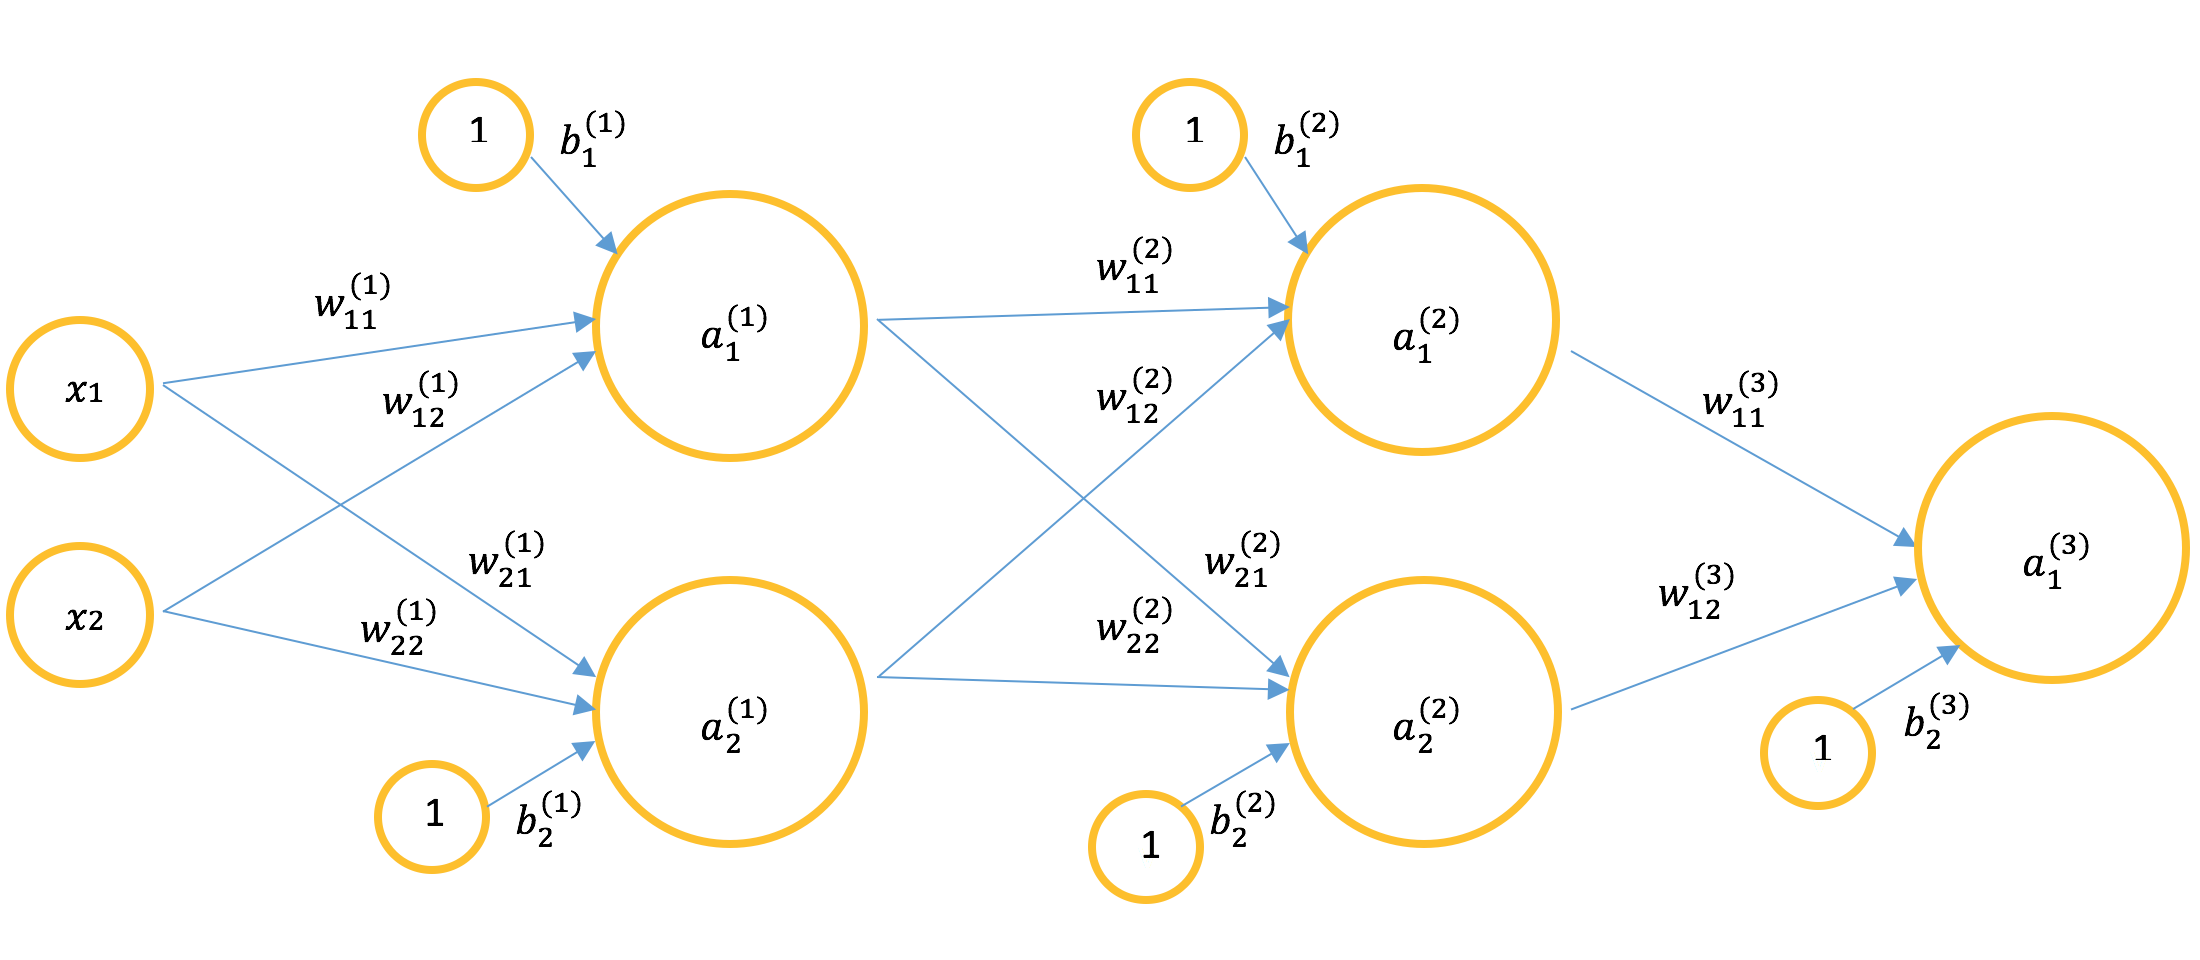
\includegraphics[scale=.3]{neural_net_image.png}
 \end{figure}
 
The notation here is important to keep straight. For the weights the number in the superscript is referring to the current layer, the first number in the subscript is referring to which node the previous node output (or feature) is going to, and the second number in the subscript is referring to which node (or feature) the current weight is coming from. So for example, $w^{(1)}_{12}$ is a weight in the first layer (because of the superscript) and connects the second feature to the first node. 

This notation comes from Nielson's book and helps when we write everything out in matrix multiplication. To see what that looks like for a given layer:

\[
\begin{bmatrix}
           z^{(1)}_{1} \\
           z^{(1)}_{2} \\
           \vdots \\
           z^{(1)}_{m}
         \end{bmatrix}
         =
\left[
  \begin{array}{cccc}
    w^{(1)}_{11} & w^{(1)}_{12} & \hdots & w^{(1)}_{1n} \\
    w^{(1)}_{21} & w^{(1)}_{22} & \hdots & w^{(1)}_{2n} \\
    \hdots &  \hdots  & \hdots &  \hdots \\
    w^{(1)}_{m1} & w^{(1)}_{m2} & \hdots & w^{(1)}_{mn} \\ 
  \end{array}
\right]
\begin{bmatrix}
           x_{1} \\
           x_{2} \\
           \vdots \\
           x_{n}
         \end{bmatrix}
+
\begin{bmatrix}
           b^{(1)}_{1} \\
           b^{(1)}_{2} \\
           \vdots \\
           b^{(1)}_{m}
         \end{bmatrix}
\]

\noindent where $n$ is the number of features, $m$ is the number of nodes, and the $z$'s are the weighted combinations. In shorthand we can write:

\begin{equation}
\mathbf{z}^{(1)} = \mathbf{W}^{(1)} \mathbf{x} + \mathbf{b}^{(1)}.
\end{equation}

One other note to make here is that the bias ($b^{(1)}$) essentially just provides a constant in our linear combination since we are only multiplying it by 1. 

Once this linear combination is fed into the node we pass it through what is known as an activation function. The purpose of this is to help our neural net model nonlinear behavior (see Deep Learning book for further discussion, pages 168-171). Another reason that Nielson points out is that we want a function that provides gradual changes with input. The original perceptron originally outputted a 0 or 1 based on if the weighted combination was greater than some threshold. This is a problem because a slight nudge in one direction could completely flip the neuron and training the network would be harder to do because of neurons that suddenly flip. Some activation functions like the sigmoid essentially approximate the perceptron paradigm (by approximating the step function) but I think the main point is that we want a function that has smoothness properties. The reason we want this is because we can approximate a change in output by a linear combination of the derivatives of the weights and bias with the actual weights and biases implying that the output is a linear function of the inputs and therefore changing parameters becomes more predictable for the algorithm to figure out.

We represent the activation function with $\sigma$ and write the output of the activation function as:
%TODO talk about activation functions here

\begin{equation}
\mathbf{a}^{(1)} = \mathbf{\sigma}(\mathbf{W}^{(1)} \mathbf{x} + \mathbf{b}^{(1)}) = \sigma(\mathbf{z}^{(1)})
\end{equation}
\noindent As Nielson points out we are treating the function $\sigma$ here as a vectorized function. A more explicit way to write this out would be:

\[
\begin{bmatrix}
           a^{(1)}_{1} \\
           a^{(1)}_{2} \\
           \vdots \\
           a^{(1)}_{m}
         \end{bmatrix}
         =
\left[
  \begin{array}{cccc}
    \sigma(w^{(1)}_{11}x_1 & w^{(1)}_{12}x_2 & \hdots & w^{(1)}_{1n}x_n + b_1^{(1)}) \\
    \sigma(w^{(1)}_{21}x_1 & w^{(1)}_{22}x_2 & \hdots & w^{(1)}_{2n}x_n + b_2^{(1)} ) \\
    \hdots &  \hdots  & \hdots &  \hdots \\
    \sigma(w^{(1)}_{m1}x_1 & w^{(1)}_{m2}x_2 & \hdots & w^{(1)}_{mn}x_n + b_m^{(1)} ) \\ 
  \end{array}
\right]
\]

To continue this notation with each subsequent layer we really only need to change a few things. First of all, instead of the original features $x_1, x_2, ..., x_n$ we have $a^{(1)}, a^{(2)}, ..., a^{(m)}$ as the inputs into the next layer. This leads us to change our weight matrix as well so that we have a matrix that is $p$x$m$ where $p$ is the number of nodes in the second layer and $m$ is the number of outputs from layer 1 (before we had $n$ representing the number of \emph{features}). The other thing we need to change is the superscript for the variables such as $\mathbf{W}^{(1)}$ to $\mathbf{W}^{(2)}$ since we are in the second layer. For a generic layer from Nielson's book we can write:

\begin{equation}
\mathbf{z}^{(l)} = \mathbf{W}^{(l)} \mathbf{a}^{(l-1)} + \mathbf{b}^{(l)}.
\end{equation}
\noindent This leads us to also write:

\begin{equation}
\mathbf{a}^{(l)} = \mathbf{\sigma}(\mathbf{z}^{(l)}).
\end{equation}

When designing our networks one heuristic that Nielsen points out is to set the number of nodes to a quantity that actually makes sense. For example, in the recognizing handwritten letters case it is better to have 10 output nodes for digits $0,...,9$ than 4 output nodes outputting a 1 or a 0 (which would allow us to treat the nodes as bits in representing numbers). The first approach might be better because it is directly tied to the images - the output node representing 0 for example should hopefully find information from the other nodes directly from the image to make decisions.


\subsection{Backprop}

Now that we have our notation straight we can talk about how the network is trained using backpropagation. Really at the heart of the backprop algorithm is gradient descent or some iterative optimization technique. To use gradient descent or similar techniques we need to calculate the partial derivatives of what is known as the cost or loss function with respect to the parameters in the model or in the case of neural networks, the weights and biases. Because the neural network is made up of different layers or functions then what this amounts to is using the chain rule for each parameter.

Nielsen brings up two good points with regards to the loss function. Take the common loss function called the mean squared error loss function:

\begin{equation}
C = \frac{1}{2n} \sum_i (y_i - a^{L}(x_i))^2
\end{equation}

First of all, the overall loss function needs to be able to be written as an average of the loss function of separate training examples. This is because backprop is designed to operate one training example at a time (giving us gradients for each training example) and the overall gradient can be recovered by averaging over all the gradients from the training examples as long as our loss function is an average to begin with over all training examples. In practice, averaging the gradient over all training examples is not usually done but instead updates happen in smaller batches called ``mini batches" over a random subset of the data (called stochastic gradient descent).

The second assumption is that the loss function can be written as a function of the outputs of the network. This is just making the point that we want to be able to train the parameters of the model and so the loss function needs to be a function of those parameters.
 
In my mind, it makes sense to think of backprop as a means to an end, in particular finding the gradient at a particular training example. To see this I calculate a partial derivative by hand below and later look at the backprop equations.

 Using our example and notation, lets find the derivative of the function with respect to the weight $w^{(1)}_{12}$. In other words we want to find:
 
 \begin{equation}
\frac{dC_{x_i}}{dw^{(1)}_{12}}.
 \end{equation}
 
\noindent where $C_{x_i}$ is referring to the loss function for a specific training example.
 
\noindent The squared-error loss function for our 3 layered network gives us:
 
 \begin{equation}
 C_{x_i} = \frac{1}{2} {(y_i - a_1^{(3)})^2}
 \end{equation}
 
 \noindent where $a_1^{(3)}$ is the output from the last layer in our example. Note that we are doing this for one particular training example. 
 
 To get at the derivative for $w^{(1)}_{12}$ we rewrite the cost function above with all its nested functions:
 
 \begin{equation}
 \begin{split}
 \frac{1}{2} (y_i - a_1^{(3)})^2 & = \frac{1}{2} (y_i - \sigma(w^{(3)}_{12}a_2^{(2)} + w^{(3)}_{11}a_1^{(2)}+ b_2^{(3)}))^2 \\
 &= \frac{1}{2} (y_i - \sigma(w^{(3)}_{12} \sigma(w^{(2)}_{22}a_2^{(1)} + w^{(2)}_{21}a_1^{(1)}+ b_2^{(2)}) + w^{(3)}_{11}        \sigma(w^{(2)}_{12}a_2^{(1)} + w^{(2)}_{11}a_1^{(1)}+ b_1^{(2)}) + b_2^{(3)}))^2 \\
 &= \frac{1}{2} (y_i - \sigma(w^{(3)}_{12}     \sigma(w^{(2)}_{22}   \sigma(w_{22}^{(1)}x_2 + w_{21}^{(1)}x_1 + b_2^{(1)})    + w^{(2)}_{21}        \sigma(w_{12}^{(1)}x_2 + w_{11}^{(1)}x_1 + b_1^{(1)})+ b_2^{(2)}) \\
 &+ w^{(3)}_{11}        \sigma(w^{(2)}_{12}  \sigma(w_{22}^{(1)}x_2 + w_{21}^{(1)}x_1 + b_2^{(1)})  + w^{(2)}_{11} \sigma(w_{12}^{(1)}x_2 + w_{11}^{(1)}x_1 + b_1^{(1)})+ b_1^{(2)})     + b_2^{(3)}))^2
 \end{split}
 \end{equation}

We then use the chain rule to get:

\begin{equation}
\frac{dC}{dw^{(1)}_{12}} = (y_i - a_1^{(3)})(-\sigma^\prime(z_1^{(3)}))[w_{12}^{(3)}\sigma^\prime(z_2^{(2)})w_{21}^{(2)}\sigma^{\prime}(z_1^{(1)})x_2 + w_{11}^{(3)}\sigma^{\prime}(z_1^{(2)})w_{11}^{(2)}\sigma^{\prime}(z_1^{(1)})x_2].
\end{equation}

We can do this for all partial derivatives with respect to our parameters (the weights and biases) giving us our gradient $\nabla C_{x_i}$ which is used in the gradient descent equation:

\begin{equation}
\theta_t = \theta_{t-1} + \eta \left( -\nabla C_{x_i}(\theta_{t-1}) \right).
\end{equation}
In this equation $\theta_t$ represents the parameters to the neural network at iteration $t$, $C_{x_i}$ represents our cost function for training example $i$, and $\eta$ is the learning rate. This update equation implies that we are updating after each training example which might not be ideal.

It is key to remember that we are treating the loss function as a function of $\theta$ and keeping everything else fixed. The goal is to find the $\theta$ that minimizes the overall loss function.







As we can see from the previous section, the algebra for this can get lengthy and messy. A key turning points for neural networks was finding a quicker way of calculating partial derivatives. 

In terms of the same weight we found above ($w^{1}_{12}$) we have the four backprop equations. Equation 1 is the error of the $j^{th}$ node in the last layer:

\begin{equation}
\delta^{L}_j = \frac{dC}{da^L_j} \sigma^\prime(z_j^L)
\end{equation}

\noindent Breaking this down we see that the first quantity on the right side of the equation is letting us know how fast the cost function is changing with respect to the output of the $j^{th}$ node. If this is high, then we know that the cost function is still fluctuating rapidly along this direction and we aren't at a minimum yet with respect to that direction. In this sense we can think of $\delta{L}_j$ referring to the error of the node. We can also write this all in vectorized form $\delta^{L}$.




\begin{equation}
\frac{dC}{dw^{(1)}_{12}} = a_{2}^{0}\delta_1^{(1)}
\end{equation}

The quantity $\delta_1^{(1)}$ is given by:

\begin{equation}
(w_{11}^{(2)}\delta^{(2)}_1 + w_{21}^{(2)}\delta^{(2)}_2)\sigma^{\prime}(z_1^{(1)})
\end{equation}
 
 We then recursively get the other $\delta$'s in the equation:
 
 \begin{equation}
 \begin{split}
 \delta^{(2)}_1  & = w_{11}^{(3)}\delta_1^{(3)}\sigma^{\prime}(z_1^{(2)})\\
 \delta^{(2)}_2  & = w_{12}^{(3)}\delta_1^{(3)}\sigma^{\prime}(z_2^{(2)})
 \end{split}
 \end{equation}
 

 
 
 For me, the best way to understand how a neural net works is to look at an actual network and learn by example. One of the classic examples is the XOR function. A discussion of this problem can be found in the Deep Learning book on pg. 167.

Figure \ref{fig:xor} shows what the data looks like for this problem. We have two features, $x_1$ and $x_2$, that can take on two possible values, 0 or 1. We assign another binary variable $y$ to each of the possible combinations of $x_1, x_2$ resulting in $(0,0) = 0, (0,1)=1, (1,1)=1, (1,0)=0$.

The goal here is to find a line that separates the response variable $y$ between its two possible values, 0 or 1. As we can see from the picture this is not possible with the current setup.

 \begin{figure} \label{fig:xor}
\caption{XOR problem}
\centering
 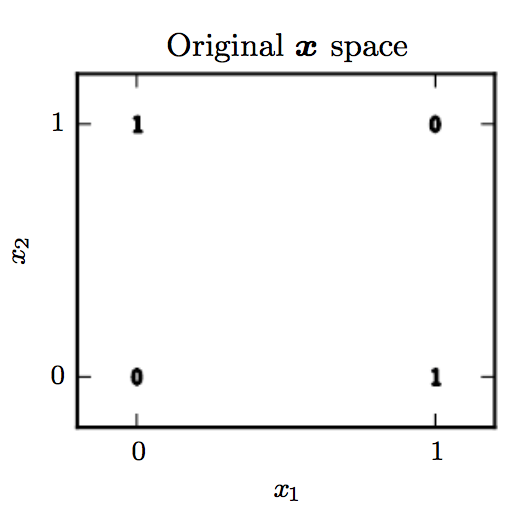
\includegraphics[scale=.7]{xor.png}
 \end{figure}
 


 
 
 
 \subsection{Recurrent and Recursive Nets}
 
(Notes from Deep Learning Book)

\begin{itemize}
\item Recurrent Nets (RNNs) are built to handle a sequence of values $\mathbf{x}^{(1)},..., \mathbf{x}^{(\tau)}$
\item Main idea is of sharing parameters across different parts of the model which allows us to deal with different sequence lengths. This is contrasted with a regular neural network which would have a separate parameter for each word position in a sentence. If the sentence has the same meaning, but is out of order we could get a totally different answer.
\item A related idea for sharing parameters is by using a neighborhood around the \emph{inputs}. With RNNs however each member of the output is a function of previous members of the \emph{output}.
\item We define hidden units as $\mathbf{h}^{(t)} = f(\mathbf{h}^{(t-1)}, \mathbf{x}^{(t)}; \theta)$. If we are trying to predict the future from the past (predict the next word given a sequence of words) then $\mathbf{h}^{(t)}$ provides a type of lossy summary of the previous inputs up to $t$. 

\item Teacher forcing is where you take the target value of one time step and input it into the next time step

\end{itemize}
 